% focusing on the second source of uncertainty here
	In Chapter~1 we identified two main sources of uncertainty affecting the execution of tasks, or activities, within the NedTrain maintenance workshop.
	In the first part of the thesis we focused on uncertainty originating in giving actors some room to decide, just-in-time, the exact dispatching time of their tasks,
	according to an unknown decision process.
	In the second part of this thesis we eliminate the source of uncertainty investigated in the first part
	by assuming actors behave deterministicaly and follow an earliest start dispatching strategy.
	That is, we assume actors will always choose to dispatch a task immediately when it becomes possible under certain constraints imposed by the dispatching process. 
	At the same time, in the second part of this thesis we focus on the other major source of uncertainty,
	which we identified in Chapter~1 to stem from our inability to predict the actual time needed for the execution of a task.
	In other words, uncertainty now stems from tasks having unpredictable durations, while actors behave predictably. 

% what are stochastic task networks 
	In Part II we shall focus on problems related to dispatching stochastic task networks, also known as stochastic activity networks.
	Such a network is typically a directed acyclic graph, the nodes of which represent tasks (or activities) with \emph{random durations}, the probability distributions of which are given.
	A directed edge between two tasks specifies a \emph{precedence constraint}. 
	Such constraints dictate that a task may only get dispatched after all its \emph{predecessors} (i.e. tasks with an outgoing arc to it) have finished.
	Such networks have been used in various domains where there is a need to model a partial order of events with random durations.
	An early application of the concept lead to the so-called \emph{PERT networks} \cite{malcolm1959}, 
	for modelling projects executed in an uncertain environment.

% stochastic makespan
	As in scheduling we usually seek to optimize efficiency, 
	a very common objective is that of minimizing \emph{makespan} -- the overall completion time of a project, or collection of tasks.
	As such, task networks is typically associated with the \emph{earliest-start dispatching} strategy,
	which amounts to simply starting a task immediately when its predecessors finish.
	Owing to the randomness of task durations,
	dispatching times and completion times of tasks are random variables.
	Clearly, then makespan, which equals the maximum of all completion times, is also a random variable.
	Moreover, its probability distribution depends on exactly the following elements:
	$i$) the task duration distributions, 
	$ii$) the network structure and $iii$) the dispatching strategy.

% task networks - mathematically 
	Mathematically, a stochastic task network can be described as a tuple $\langle G=(V,E), D \rangle$.
	Here, $G$ is the directed graph of precedence constraints with $V=\{1,\ldots,n\}$ the indices of tasks 1 to n and $E \subseteq V\times V$ the set of directed arcs.
	Element $D=(D_1,\ldots,D_n)$ is a random vector, such that random variable $D_i$ represents the duration of task $i$.
	We shall use $\mathbb{P}[D_i = d_i]$ to denote the probability of observing realization $d_i$ of random variable $D_i$.
	The joint probability distribution $\mathbb{P}[D_1=d_1, \ldots, D_n=d_n]$ of vector $D$, is given.
	For simplicity, it is usually assumed that variables $D_i$ are independent.
	As such, the joint distribution of $D$ typically evaluates to $\prod_{i} \mathbb{P}[D_i=d_i]$ and we are, in fact, 
	given the individual distribution of each duration variable. 
	If we use $S_j$ to denote the (random) dispatching time of task $j$,
	then earliest start dispatching yields:
	\begin{align}
		S_j := \max \{S_i + D_i : i \textrm{ is a predecessor of } j\} \label{chapter:prelim-2:sj}
	\end{align}
	That is, task $j$ is dispatched immediately when all its predecessors finish (clearly, the finish time of task $i$ is equal to $S_i + D_i$).

	\begin{figure}
		\centering
		\begin{tikzpicture}
			\tikzset{vertex/.style = {shape=circle,draw,minimum size=1.5em}}
			\tikzset{edge/.style = {->,> = latex'}}
			\node[vertex,label={\scriptsize $[2,4]$}] (1) at (0,0)			{\small $1$};
			\node[vertex,label={\scriptsize $[4,7]$}] (2) at (1.5,1)			{\small $2$};
			\node[vertex,label={\scriptsize $[2,4]$}] (3) at (1.5,-1)		{\small $3$};
			\node[vertex,label={\scriptsize $[2,3]$}] (4) at (3,0)			{\small $4$};
			\node[vertex,label={\scriptsize $[2,3]$}] (5) at (3,-2)			{\small $5$};
			\draw[edge] (1) to[] (2);
			\draw[edge] (1) to[] (3);
			\draw[edge] (3) to[] (4);
			\draw[edge] (3) to[] (5);
		\end{tikzpicture}
		\caption{Task network consisting of precedence constraints over five tasks with uncertain durations.
		Each task is annotated with the interval within which its duration is expected to vary.}
		\label{chapter:prelim-2:example-1}
	\end{figure}


	\begin{example}
		Consider the example task network displayed in Figure~\ref{chapter:prelim-2:example-1},
		illustrating a hypothetical situation with five maintenace operations to be performed in the NedTrain workshop, subject to precedence constraints.
		Tasks 2 and 3 cannot start before the completion of task 1 and similarly, tasks 4 and 5 cannot start before the completion of task 3.
		Assuming earliest start dispatching and that task 1 starts at time 0 (i.e. $S_1 = 0$), we derive the following equations
		\begin{align*}
			S_2 & = S_3 = S_1 + D_1 \\
			S_4 & = S_5 = S_3 + D_3 
		\end{align*}
		The duration $D_j$ of each task $j$ is uncertain, but from data collected over past maintenance sessions,
		we are able to bound the duration of each task with a minimum and a maximum number of hours.
		This is indicated here by annotating each node with the interval within which its duration is expected to vary.
		That is, task 1 will take between 2 and 4 hours, task 2 between 4 and 7 hours, and so on.%
		\footnote{Note that annotating nodes with duration intervals as we do here is not standard practice in the literature.}%
		For now, we shall make no assumptions regarding the probability distribution of each task duration.
		But since durations are bounded by minimum and maximum values (which may not be the case in general),
		using earliest-start dispatching, the resulting makespan may vary between 6 and 11 hours, depending on the realized scenario.
		This is better illustrated in Figure~\ref{chapter:prelim-2:example-1b} which presents two marginal cases of the realized schedule.
		Figure~\ref{chapter:prelim-2:example-1b} examines two marginal scenarios:
		On the upper (lower) side, the outcome schedule is presented when earliest start dispatching is used and 
		when each task duration takes its minimum (maximum) value.
	\end{example}

	\begin{figure}
		\centering
		\begin{subfigure}[b]{0.7\textwidth}
			\begin{ganttchart}[vgrid,
				x unit=0.5cm,
				y unit chart=0.5cm,
				y unit title=0.5cm,
				title label font=\scriptsize,
				bar label font=\footnotesize,
				bar/.style={draw=gray, fill=white, rounded corners=1pt}
				]{0}{12}
				\gantttitlelist{0,...,12}{1} \\
				\ganttbar{Task 1}{1}{2}  \\
				\ganttbar{Task 2}{3}{6} \\
				\ganttbar{Task 3}{3}{4} \\
				\ganttbar{Task 4}{5}{6} \\
				\ganttbar{Task 5}{5}{6} 
			\end{ganttchart}
			\subcaption{Resulting schedule with minimum task durations.}
			\label{chapter:prelim-2:example-1b-a}
		\end{subfigure}
		
		\vspace{10pt}

		\begin{subfigure}[b]{0.7\textwidth}
			\begin{ganttchart}[vgrid,
				x unit=0.5cm,
				y unit chart=0.5cm,
				y unit title=0.5cm,
				title label font=\scriptsize,
				bar label font=\footnotesize,
				bar/.style={draw=gray, fill=white, rounded corners=1pt}
				]{0}{12}
				\gantttitlelist{0,...,12}{1} \\
				\ganttbar{Task 1}{1}{4}  \\
				\ganttbar{Task 2}{5}{11} \\
				\ganttbar{Task 3}{5}{8} \\
				\ganttbar{Task 4}{9}{11} \\
				\ganttbar{Task 5}{9}{11} 
			\end{ganttchart}
			\subcaption{Resulting schedule with maximum task durations.}
			\label{chapter:prelim-2:example-1b-b}
		\end{subfigure}

		\caption{Earliest start dispatching in two marginal scenarios.}
		\label{chapter:prelim-2:example-1b}
	\end{figure}

% the makespan distribution problem
\section{The makespan distribution problem}
	Always assuming earliest-start dispatching and since the appearance of PERT networks a few decades ago,
	research is still in progress concerning the problem of computing the makespan distribution.
	Makespan, as a variable, is usually denoted as $C_{max}$ (representing the $max$imum $C$ompletion time of a task in the project) and is defined as:
	\[
		C_{max} := \max\{ S_i + D_i : i \in V\}
	\]
	i.e. as the latest completion time of a task. 
	Knowing the distribution $\mathbb{P}[C_{max} = t]$ is important for obvious reasons,
	since it amounts to knowing the expected project completion time,
	the chance of finishing the project by a certain due-date and so on. 
	As shown by Hagstrom in \cite{hagstrom1990},
	assuming duration distributions $\mathbb{P}[D_i = d]$ have finite and discrete support,
	computing the probability distribution of $C_{max}$ or even its expectation $\mathbb{E}[C_{max}]$ is an intractable problem.
	As such, most approaches in the literature are heuristic.
	Quite often, approximating the makespan distribution involves Monte Carlo simulation based on a sample of task durations.

	\begin{example}
		Let us now assume that duration of each task from our earlier example varies (within the given bounds)
		according to the Beta distribution with parameters $\alpha = 2, \beta = 1.5$.
		Figure~\ref{chapter:prelim-2:example-1b-a} shows a histogram obtained by sampling the distribution of the duration of task 2, which ranges between 4 and 7 hours.
		Our choice of parameters $\alpha$ and $\beta$ results in a forward skew which indicates a certain degree of pessimism,
		as we expect the duration of each task to be realized closer to its maximum value.
		Figure~\ref{chapter:prelim-2:example-1b-b} shows a histogram obtained by sampling the distribution of makespan,
		which as we saw earlier will vary between 6 and 11 hours.
		Visual inspection of the histogram reveals that completing all the tasks in the network is unlikely to take less than 8 hours or more than 10 hours.
		Using such a makespan histogram, a due-date with arbitrarily high chances of being met can be readily determined.
	\end{example}

	\begin{figure}
		\centering
		\begin{subfigure}[b]{0.45\textwidth}
			\centering
			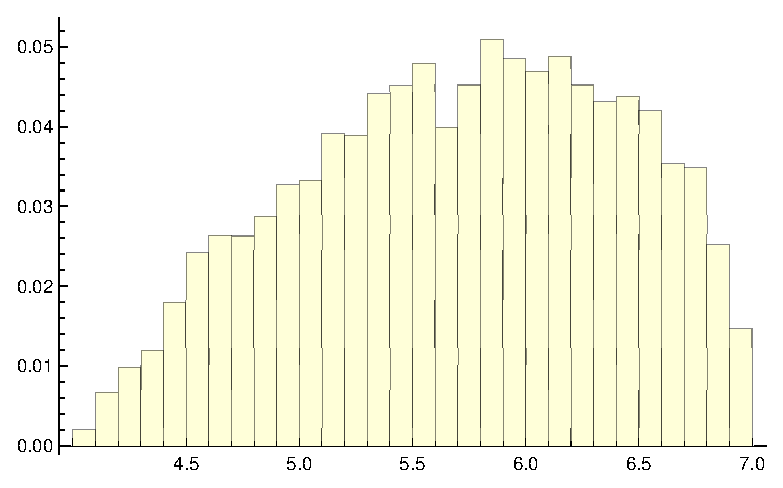
\includegraphics[width=0.95\textwidth]{chapter/prelim-2/D2}
			\subcaption{}
			\label{chapter:prelim-2:example-2-a}
		\end{subfigure}
		\quad
		\begin{subfigure}[b]{0.45\textwidth}
			\centering
			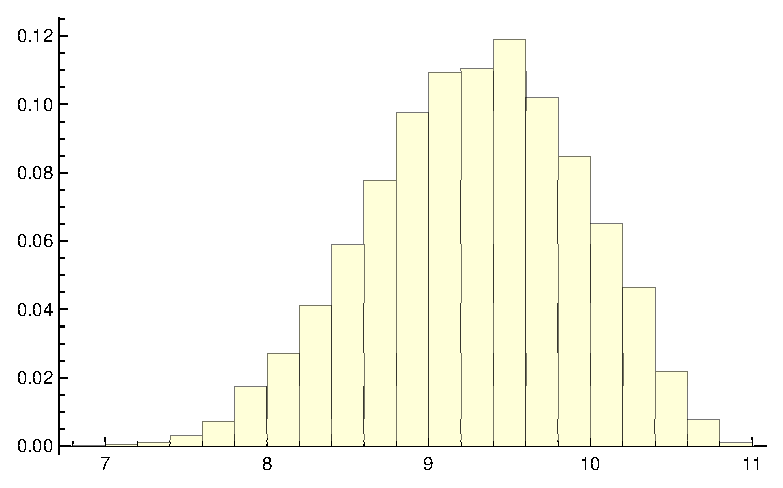
\includegraphics[width=0.95\textwidth]{chapter/prelim-2/cmax}
			\subcaption{}
			\label{chapter:prelim-2:example-2-b}
		\end{subfigure}
		\caption{Sampling the distribution of task 2 (a) and the makespan distribution (b).}
		\label{chapter:prelim-2:example-2}
	\end{figure}

	Obtaining such a histogram `approximation' of the makespan distribution can be accomplished with the following straightforward process.
	First, a topological order of the task network is computed with an algorithm like \cite{tarjan1976}.
	Then, a sufficiently large number of realizations (or scenarios) of random vector $D=(D_1,\ldots,D_n)$ is generated,
	which can be trivial when $D_i$ are independent random variables.
	Finally, the realized schedule for each generated scenario can be computed with Eq.~\ref{chapter:prelim-2:sj} by visiting each task in topological order.
	
% the pert problem in vlsi design
	\subsection{The makespan distribution problem in VLSI}
	In addition to project scheduling, 
	computing the makespan distribution turns out to be important in the design of Very Large Scale Integration (VLSI) circuits.
	This problem emerges because a digital circuit can be modelled as a stochastic task network.
	Nodes correspond to gates (instead of tasks) and precedence constraints corresponding to wiring.
	The equivalent of a task duration is now the amount of time needed by a gate to prepare its output.
	Due to manufacturing imperfections, the latter varies randomly across the chip surface,
	and under certain conditions we may assume to know its probability distribution.
	Makespan corresponds to the length of the clock cycle and computing its distribution
	allows us to compute the \emph{yield} -- the probability that a certain percentage of manufactured chips satisfy certain timing criteria.

	Computing the makespan distribution has received significant additional attention
	since the relatively recent discovery of its important role in the industry of circuit design \cite{blaauw2008}.
	The continuously growing area of so-called \emph{Statistical Timing Analysis} (STA) includes
	a variety of efficient techniques for accurately estimating the distribution of networks with millions of nodes.
	STA techniques range from propagating analytical expressions of the distribution through the network \cite{visweswariah2006}
	to sophisticated Monte Carlo sampling \cite{veetil2011}.
	The use of STA techniques in large-scale project scheduling problems has been studied at least in \cite{mountakis2013}.

% scheduling policies
\section{Scheduling policies}
	Turning our attention back to scheduling,
	in some applications tasks occuppy certain amounts of one or more resources during their execution.
	The resource demands of tasks and the capacities of available resources are known together in scheduling as \emph{resource constraints}.
	Note that one or more tasks which are not precedence-related may execute in parallel.
	Such a combination of tasks the total resource demands of which would exceed resource capacities in case they overlapped in time, 
	is often known as a \emph{forbidden set}.
	For a more comprehensive summary of resource constraints,
	the reader may refer to Section~\ref{chapter:prelim-1:resource-constraints}.
	
	\begin{example}
		Consider the example task network in Figure~\ref{chapter:prelim-2:example-1} and assume, 
		for tasks 2,4 and 5, that each requires the use of a repair platform during its execution.
		If in addition we assume there are only two platforms available, then tasks 2, 4 and 5 form a forbidden set.
		Consider the two schedules formed by earliest start dispatching and shown in Figure~\ref{chapter:prelim-2:example-1b}.
		Neither schedule is feasible as both allow the three tasks to overlap within intervals $[5, 6]$ and $[9, 11]$, respectively,
		over-subscribing to the repair platform resource.
	\end{example}

	Given a stochatic task network along with resource constraints,
	an emerging problem is to define a dispatching strategy that minimizes \emph{expected makespan} while preventing a forbidden set from overlapping during execution,
	ensuring the realized schedule satisfies both precedence and resource constraints.
	Note that earliest-start dispatching is generally not such a strategy, 
	since it only accounts for precedence constraints.
	M\"ohring et al. have studied possible classes of such dispatching strategies,
	known as \emph{scheduling policies} \cite{mohring1984stochastic,mohring1985stochastic}.%
	\footnote{From this point on, the terms scheduling policy and dispatching strategy shall be used interchangeably.}
	A computational study examining the potential superiority of certain classes was conducted by Stork in \cite{stork2000branch}, 
	based on exact branch-and-bound procedures.
	Recently, a new exact method was proposed in \cite{creemers2015minimizing} and
	other authors investigated (meta-)heuristics for minimizing expected makespan \cite{ashtiani2011new, ballestin2009resource}.

% es-policies and partial order schedules 
	We have already encountered a class of scheduling policies, back in Chapter~\ref{chapter/prelim-1}.
	More specifically, in Section ~\ref{chapter:prelim-1:resource-constraints} we discussed how given a network of termporal constraints along with resource constraints,
	we can eliminate forbidden sets by adding precedence constraints to form a so-called partial order schedule (or POS for short).
	Partial order schedules are almost identical to so-called \emph{earliest start policies}.
	The difference between an earliest start policy and a partial order schedule is subtle.
	Partial order schedules are discussed in the context of STP constraints between pairs of tasks,
	while earliest start policies are discussed in the context of simple precedence constraints.
	Just as a network of precedence constraints is a special case of a STP, 
	it could be argued, then, that an earliest start policy is a special-case of a partial order schedule.
	We demonstrate the concept of an earliest start policy with the following example.

	\begin{example}
		In our previous example, we saw that tasks 2, 4 and 5 form a forbidden set and as such,
		their execution should not overlap at any point in time in a feasible schedule.
		To prevent these tasks from overlapping, 
		it suffices to add a precedence constraint between any two members of the forbidden set $\{2,4,5\}$.
		Recall that a precedence constraint is a directed arc $(i, j)$, meaning that $j$ has to wait for the completion of $i$.
		Adding any of the constraints enumerated below would turn our example task network into an earliest start policy,
		the dispatching of which is guaranteed to produce a schedule satisfying both precedence and resource constraints, regardless of outcome task durations.
		\begin{enumerate}
			\item $(2,4)$, yielding an expected makespan of 11.4 hours
			\item $(4,2)$, yielding an expected makespan of 14.5 hours
			\item $(2,5)$, yielding an expected makespan of 11.4 hours
			\item $(5,2)$, yielding an expected makespan of 14.5 hours
			\item $(4,5)$, yielding an expected makespan of 11.4 hours
			\item $(5,4)$, yielding an expected makespan of 11.4 hours
		\end{enumerate}
		Note that without adding any of the constraints listed above, we observe an expected makespan of 9.2 hours.
		Clearly, delaying the dispatching of task 2 (by adding either $(4,2)$ or $(5,2)$) is not preferrable, 
		as it results in the largest expected makespan increase.
	\end{example}

% the concept of stability
\section{Stability and robustness}
\label{chapter:prelim-2:stability}
	Dispatching a stochastic task network (with a scheduling policy) in order to minimize expected makespan 
	is said to maximize \emph{quality-robustness}, or simply robustness.
	All works cited so far focus on finding a policy of optimal quality-robustness.
	Optimizing quality-robustness alone, however, is not always a suitable objective.
	Next to quality robustness,
	in certain applications it is also important to have a \emph{predictive schedule} 
	from which the realized schedule is not expected to deviate too far.
	Without such a predictive schedule offering visibility into the future,
	human and other types of resources cannot plan ahead in order to be in the right place, at the right time.
	The quality of such a predictive schedule to remain close to the realized schedule
	is often known in scheduling literature as \emph{solution-robustness} or \emph{stability} \cite{bidot2009, van2006trade}.

	\begin{example}
		Figure~\ref{chapter:prelim-2:example-3-a} shows (a histogram of) the resulting dispatching times for tasks 2, 3, 4 and 5 
		of the network in Figure~\ref{chapter:prelim-2:example-1} when using earliest start dispatching 
		and assuming durations follow the Beta distribution as described earlier.
		The dispatching time of task 1 is ommitted, as it has no predecessors to wait for and can thus always start at time 0.
		Clearly, the outcome dispatching times are rather unpredictable.
		Task 4, for instance, may start anywhere between time 4 and 8,
		with each of the possible start times having a chance of at most 10\% of being observed.
		It is therefore impossible to plan ahead for the participation of human and other types of resources.
	\end{example}

	The unpredictability of future dispatching times in the workshop can, in fact, be controlled
	with an approach sometimes known as \emph{railway scheduling} \cite{van2005use}.
	Given a task network and a scheduling strategy (if resource constraints are present),
	this approach amounts to defining a predictive dispatching time, per task, and 
	modifying the dispatching process to force the outcome dispatching times to remain close to predictive ones.
	More in particular, each task $j$ is associated with a respective predictive dispatching time $t_j$.
	Whatever dispatching strategy is in use must then observe this additional restriction:
	task $j$ may not be dispatched before $t_j$, even if doing so would not violate any temporal or resource constraints.
	%In case of earliest start dispatching (e.g. when no resource constraints are given, or when using an earliest start policy),
	%instead of starting a task $j$ immediately when its predecessors finish (i.e. according to Eq.~\ref{chapter:prelim-2:sj}),
	%we would also account for its associated predictive schedule time $t_j$, as follows:
	%\begin{align}
	%	S_j := \max \left\{ t_j, \max \{S_i + D_i : i \textrm{ is a predecessor of } j\}  \right\} \label{chapter:prelim-2:sj-stable}
	%\end{align}

	\begin{figure}
		\centering
		\begin{subfigure}[b]{0.95\textwidth}
			\centering
			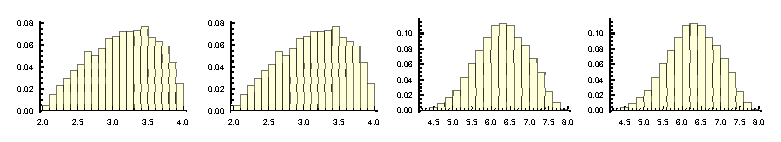
\includegraphics[width=0.95\textwidth]{chapter/prelim-2/row1}
			\subcaption{No predictive schedule.}
			\label{chapter:prelim-2:example-3-a}
		\end{subfigure}
		
		\begin{subfigure}[b]{0.95\textwidth}
			\centering
			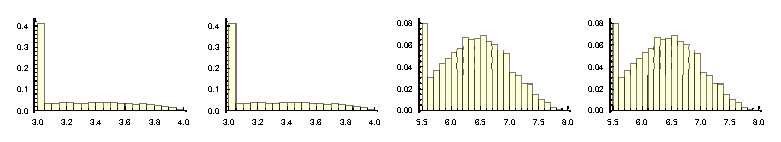
\includegraphics[width=0.95\textwidth]{chapter/prelim-2/row2}
			\subcaption{Using predictive schedule $t_1 = 0, t_2 = 3.0, t_3 = 3.0, t_4 = 5.5, t_5 = 5.5$.}
			\label{chapter:prelim-2:example-3-b}
		\end{subfigure}

		\begin{subfigure}[b]{0.95\textwidth}
			\centering
			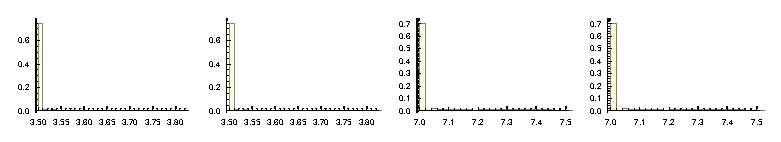
\includegraphics[width=0.95\textwidth]{chapter/prelim-2/row4}
			\subcaption{Using predictive schedule $t_1 = 0, t_2 = 3.5, t_3 = 3.5, t_4 = 7.0, t_5 = 7.0$.}
			\label{chapter:prelim-2:example-3-c}
		\end{subfigure}
		\caption{Histogram representation of the realized dispatching times for tasks 2, 3, 4 and 5 (with task 1 always dispatched at time 0) for our example task network,
		when using earliest start dispatching with and without a predictive schedule.
		As predictive start times are spread farther apart, start time variability diminishes.}
		\label{chapter:prelim-2:example-3}
	\end{figure}

	As better illustrated in the following example,
	as those predictive (or minimum) start times are spread along the time-axis, 
	unpredictability diminishes (or stability improves) and outcome dispatching times tend to stay close to predictive ones.
	In effect, then, vector $(t_1, t_2, \ldots, t_n)$ constitutes a reliable predictive schedule that can be used for planning ahead.

	\begin{example}
		Figure~\ref{chapter:prelim-2:example-3-b}
		shows what happens when earliest start dispatching is used with the additional rule that
		tasks 2, 3, 4 and 5 cannot start before $t_2 = 3.0, t_3 = 3.0, t_4 = 5.5$ and $t_5 = 5.5$, respectively.
		Clearly, the start times of tasks 2 and 3 become more predictable,
		with a start time of $t_2 = t_3 = 3.0$ for tasks 2 and 3 having a relatively high chance of being observed, at 40\%. 
		Unfortunately, the start times of tasks 4 and 5 remain unpredictable.
		Figure~\ref{chapter:prelim-2:example-3-c} shows how stability improves when the predictive schedule is spread farther apart in time,
		yielding, for each task, a chance of about 70\% to start at its predictive start time.
		Moreover, note how even if a task does not start at its predictive time, it will most likely start somewhere near. 
		Tasks 4 and 5, for instance, might start with a delay of at most 0.5 hours from their predictive time.
		Enhancing stability, however, has an impact on performance.
		When not using a predictive schedule at all (i.e. Figure~\ref{chapter:prelim-2:example-3-a}) the expected makespan is at 9.2 hours.
		Using the predictive schedule in Figure~\ref{chapter:prelim-2:example-3-b}, expected makespan increases only slightly at 9.4 hours.
		Ultimately, using the stable predictive schedule in Figure~\ref{chapter:prelim-2:example-3-c} yields an expected makespan of 9.9 hours.
	\end{example}

	%When the focus is exclusively on minimizing expected makespan, however, 
	%the realized schedule (i.e. the outcome task start times) is mostly unpredictable.

	As demonstrated in our previous example,
	scheduling tasks efficiently and scheduling tasks predictably 
	(or optimizing quality-robustness and solution-robustness) are usually conflicting objectives \cite{van2006trade}.
	A relatively small research area  within the literature, known as \emph{proactive-reactive project scheduling},
	focuses on problems for which the solution is a pair formed by a scheduling policy and a predictive schedule.
	The objective is to find such a pair offering an optimal \emph{trade-off} between quality-robustness and stability.
	The work presented in Chapters 6 and 7 of this dissertation focuses on the problem of trading robustness for stability.

% research questions
\section{Research Questions}
\label{chapter:prelim-2:research-questions}
	In this Section we discuss how existing work, summarized in preceeding sections,
	can help us address Research Problem II, stated in Chapter~1.
	In doing so, we raise appropriate Research Questions that map to gaps in existing literature.
	The raised questions are eventually addressed in Chapters 6 and 7.

	% RP statement and policies as robust schedules
	Referring back to Research Problem II, 
	we would like to compute robust and stable schedules for work-teams,
	in order to deal with uncertainty in the duration of maintenance tasks.
	A robust schedule should guarantee good performance under a variety of possible outcome duration scenarios.
	Owing to the recurrent nature of maintenance operations,
	we are able to gather data over past maintenance sessions and build, for each task duration, 
	a probability distribution according to which it varies over different executions.
	Given the description of each task duration as a random variable with a known distribution,
	a scheduling policy is functionally equivalent to a robust schedule,
	as it provides a set of rules for deriving appropriate dispatching times by reacting to observed task durations,
	such that feasibility and good performance are both guaranteed over a range of possible scenarios.

	% the need for stability
	As explained in Section~\ref{chapter:prelim-2:stability}, however, robustness alone is not always sufficient.
	Next to ensuring good performance under a variety of potential scenarios and taking the human factor into account, 
	we would also like to offer stability, or visibility of future dispatching times.
	That is, we would also like to force and/or predict that outcome dispatching times will fall within certain time-windows,
	or near certain predictive dispatching times. 
	Such a stable or predictive schedule is necessary for planning-ahead the availability of human and other resources
	in the right place and at the right time in the workshop.

	% coverage by existing literature
	Modern literature on stochastic project scheduling addresses the problem of balancing robustness and stability
	with techniques for computing a scheduling policy along with a reliable predictive schedule.
	Existing approaches, however, suffer from certain limitations,
	as they tend to treat the scheduling policy and the predictive schedule separately.
	The prominent paper by Van de Vonder et al. \cite{van2008}, for instance, 
	treats the optimization of a policy and predictive schedule separately, in a-two step fashion,
	while the exact approach of \cite{lamas2015} follows a policy-agnostic approach, 
	optimizing the predictive schedule without assuming anything about the structure of the policy.
	Considering, instead, the problem as a whole such that the structure of the policy is taken into account when choosing the predictive schedule, and vice-versa,
	gives us access to a solution-space of higher dimensionality.
	Since performance is determined in practice by the policy and the predictive schedule together,
	in pursuit of potentially better results we would like to address the following question:
		
		\begin{rquest}
			\label{rquest-2-1}
			How to optimize a scheduling policy and a predictive schedule together as a pair?
		\end{rquest}

	% RP: diminishing of uncertainty
	Moreover, as time progresses and outcome dispatching times and task durations are being observed, 
	uncertainty gruadually diminishes in the workshop.
	As such, we are presented with an opportunity to adapt to new information accordingly by rescheduling.
	In order to keep pace with execution and to avoid introducing further delays,
	the computational effort spent in rescheduling should be rather limited in practice. 
	Therefore, during rescheduling we should avoid reconsidering the structure of the scheduling policy,
	in order to avoid the combinatorial explosion associated with reasoning about resource constraints.
	It might, however, be fruitful to react to new information by adapting the predictive schedule.
	As such, we are interested in addressing the following question:

		\begin{rquest} 
			\label{rquest-2-2}
			How to update the predictive schedule by reacting to outcome durations in low order polynomial time, keeping pace with execution?
		\end{rquest}

	Research Question~\ref{rquest-2-1} is answered in Chapter~6.
	In the first part of Chapter~6, we present a linear programming (LP) approach for finding a predictive schedule offering an optimal 
	trade-off between makespan and stability, given a fixed earliest start policy.
	In the second part we develop a Mixed Integer LP extension of our approach which enables 
	us to optimize an earliest start scheduling policy together with the predictive schedule.
	Research Question~\ref{rquest-2-2} is answered in Chapter~7.
	There, we present a dynamic programming algorithm which can function as a much faster alternative to the LP approach developed in Chapter 6.
